\section{注意点}
完成したら必ずこの部分はmainから削ってください

\section{倒立振子の全体の流れ}
以下に今回行った倒立振子に関する実験及びシミュレーションなどの流れを示す\\
\\
1.倒立振子のモデリングと自由応答シミュレーション(B.倒立振子の安定化制御、制御工学実験第3\ 倒立振子の安定化制御の資料も含む)\\
2.倒立振子のパラメータ同定と検証\\
3.設計(線形)モデルの決定とシステム解析\\
4.制御系の設計1(状態フィードバック)と制御性能評価\\
5.制御系の設計2(最小次元オブザーバ)と制御性能評価\\
6.制御系の設計3(コントローラの離散化)と制御性能評価\\
7.制御系の設計4(振り上げ制御・安定化)と制御性能評価\\
8.倒立振子の制御実験(安定化制御)\\
9.倒立振子の制御実験(目標値の変更)\\
10.倒立振子の制御実験(振り上げ制御・安定化)\\
11.教育機関報告書作成(その1)\\
\\
以上を分割を以下のグループに分けることで今までしてきたことがどのチャプターにかかれるかを示す\\
\\
A:はじめに\ この実験を行う背景とか\\
B:モデリング\ 1,\ 2,\ 3,\\
\\
C:制御系設計\ 4,\ 5,\ 6,\ 7\\
\\
D:シミュレーション\ 1,\ 2,\ 4,\ 5,\ 6,\ 7,\ 8,\ 9,\ 10\\
\\
E:実験\ 8,\ 9,\ 10\\
F:おわりに\ 学んだこととか\\
G:プログラム\ 

\section{疑問}
質問コーナー\\

・シミュレーションの部分は今までやってきたシミュレーションすべてを書かなければならないか\\
→最低限実験と比較したシミュレーションは必要。それ以外は任意でよい。必要最低限のせればよい\\
・制御系の設計などでMaTX,Java,JaMOXの3通りからアプローチをかけたが報告書にはそのすべてを記載末うべきか\\
→任意でよい。でもjamoxのブロック線図は乗せたほうが良い\\
・付録のプログラムについても同様で3通りのプログラムやブロック線図を貼り付けるべきか\\
→任意でよい\\
・\\
・\\
・\\
・\\
・\\
・\\
・\\
・\\
・\\
・\\
・\\

\section{トラブルシューティング}
トラブルシューティング!困ったときはここを見てね\\
・図においてlabelとrefを対応させるときにはlabelをcaptionの下に置く必要がある\\
・改ページを行うにはnewpageを用いる\\
・改段落にはparを用いる\\
\begin{figure}[h]
		\centering
		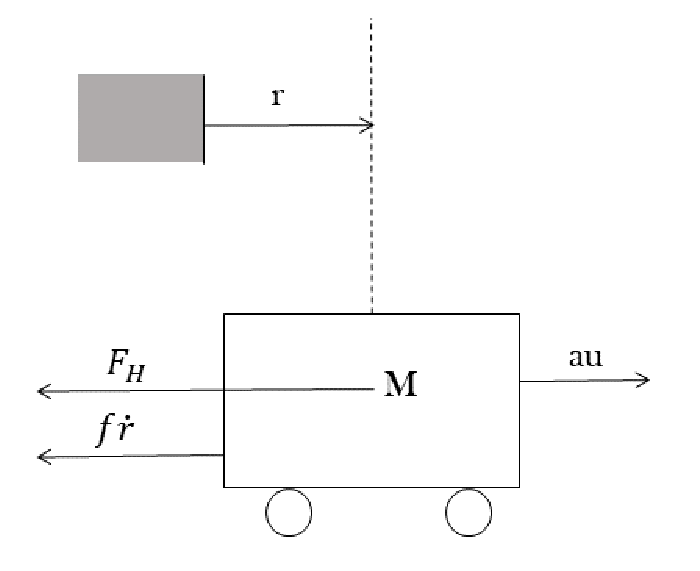
\includegraphics[width=0.4\linewidth]{gazo/cart.eps}
		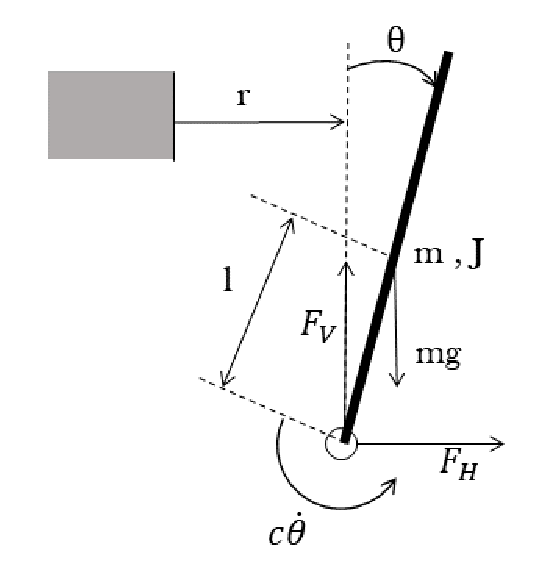
\includegraphics[width=0.4\linewidth]{gazo/stick.eps}
		\caption{数式モデル導出のための参考図}
		\label{image:test}
\end{figure}
・gnuplotでepsを出力するにはset terminal postscript epsを実行し、plotを実行すればよい\\
・報告書に使っている図と使っていない図を分ける\\
・\\
・\\
・\\
・\\
・\\

\section{TODO}
・図の矢印の線を4ptにする\\
・矢じりを塗りつぶす\\
・半角、全角を整える\\
・不要な式番号を排除する\\
・グラフの画像を見やすいように修正する\\
・\\
・\\